\let\negmedspace\undefined
\let\negthickspace\undefined
\documentclass[journal]{IEEEtran}
\usepackage[a5paper, margin=10mm, onecolumn]{geometry}
%\usepackage{lmodern} % Ensure lmodern is loaded for pdflatex
\usepackage{tfrupee} % Include tfrupee package

\setlength{\headheight}{1cm} % Set the height of the header box
\setlength{\headsep}{0mm}     % Set the distance between the header box and the top of the text

\usepackage{gvv-book}
\usepackage{gvv}
\usepackage{cite}
\usepackage{amsmath,amssymb,amsfonts,amsthm}
\usepackage{algorithmic}
\usepackage{graphicx}
\usepackage{textcomp}
\usepackage{xcolor}
\usepackage{txfonts}
\usepackage{listings}
\usepackage{enumitem}
\usepackage{mathtools}
\usepackage{gensymb}
\usepackage{comment}
\usepackage[breaklinks=true]{hyperref}
\usepackage{tkz-euclide} 
\usepackage{listings}
% \usepackage{gvv}                                        
\def\inputGnumericTable{}                                 
\usepackage[latin1]{inputenc}                                
\usepackage{color}                                            
\usepackage{array}                                            
\usepackage{longtable}                                       
\usepackage{calc}                                             
\usepackage{multirow}                                         
\usepackage{hhline}                                           
\usepackage{ifthen}                                           
\usepackage{lscape}
\begin{document}

\bibliographystyle{IEEEtran}
\vspace{3cm}
\title{1.1.6-21}
\author{EE24BTECH11028 - Jadhav Rajesh}
% \maketitle
% \newpage
% \bigskip
{\let\newpage\relax\maketitle}

\renewcommand{\thefigure}{\theenumi}
\renewcommand{\thetable}{\theenumi}
\setlength{\intextsep}{10pt} % Space between text and floats


\numberwithin{equation}{enumi}
\numberwithin{figure}{enumi}
\renewcommand{\thetable}{\theenumi}
 \textbf{Question:} Show that points A$\brak{a,b+c}$, B$\brak{b,c+a}$, C$\brak{c,a+b}$ are collinear.\\

 \solution The matrix\\
 \begin{align}
                \myvec{B-A & C-A}^{T} =
                                 \myvec{b-a & a-b\\
                                        c-a & a-c}
 \end{align}
 \begin{align}
                 C_{1}\rightarrow{C_{1}+C_{2}} \myvec{0 & a-b\\
                                                     0 & a-c}
 \end{align}
            Which has rank 1.Using rank$A$ =rank$A^{T}$ , we conclude that the given points are collinear.\\

            Define the coordinates of point A, B,, and C
 \begin{align}
             a,b,c = 1,2,3
 \end{align}

\begin{figure}[h!]
	\centering
	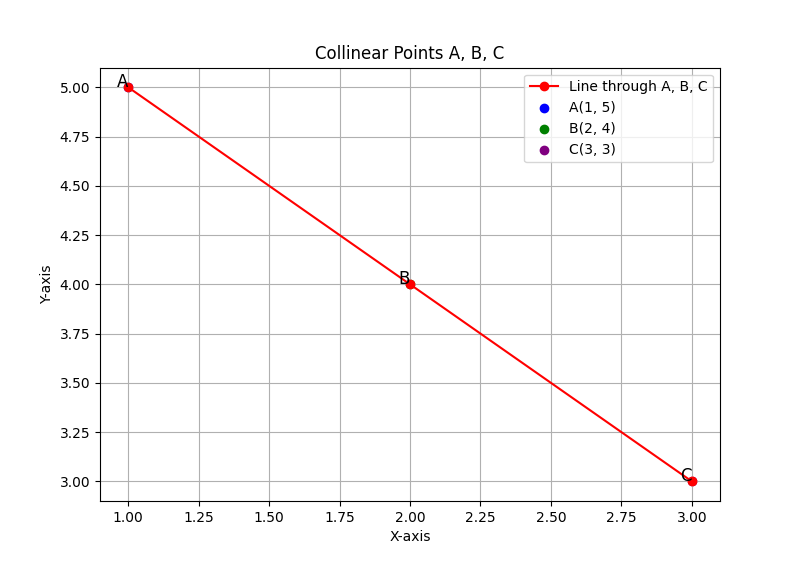
\includegraphics[width=0.5\linewidth]{Figs/Figure_1.png}
	\caption{ $\vec{A}\vec{B}\vec{C}$Collinear points}


	\label{stemplot}
\end{figure}
              

          

    
            
            
        




            
















\end{document}

